\documentclass{beamer}
\usepackage[utf8]{inputenc}
\usepackage{listings}
\definecolor{LighterGray}{rgb}{0.9,0.9,0.9}
\definecolor{LightGray}{rgb}{0.7,0.7,0.7}
\definecolor{DarkGray}{rgb}{0.4,0.4,0.4}
\lstdefinestyle{vbasic}{ %
  language=[Visual]Basic,%
  basicstyle=\ttfamily\footnotesize,
  breakatwhitespace=false,%
  commentstyle=\color{DarkGray},%
  breaklines=true,%
  keywordstyle=\color{blue},%
  showspaces=false,
  showstringspaces=false,
  showtabs=false,
  numbers=left,
  numbersep=5pt,
  numberstyle=\tiny\color{LightGray},
  stringstyle=\color{orange}
}
\usetheme{Ilmenau}
\setbeamertemplate{navigation symbols}{}
\setbeamertemplate{footline}[page number]{}
\title{Visual Basic}
\titlegraphic{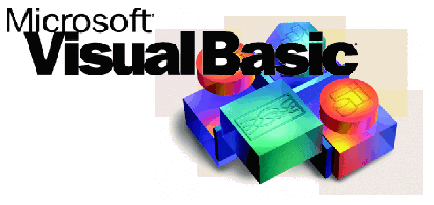
\includegraphics[scale=0.55]{VisualBasicLogo.png}}
\author{Héctor Ramón}
\date{4 de juny 2014}
\begin{document}
\frame{\titlepage}
\begin{frame}{Introducció}
\begin{description}
\item[Paradigma]
\emph{Event-driven} i \emph{object-based}
\item[Desenvolupat per]
Microsoft
\item[Dates]
1991 (presentació), 1998 (última versió)
\item[Utilitat]
Desenvolupament ràpid d'aplicacions amb interfície gràfica d'usuari
\item[Influenciat per]
BASIC, QuickBASIC
\end{description}
\end{frame}
\begin{frame}[fragile]{Característiques}
\begin{description}
\item[IDE propi]
Dissenyador de GUIs, editor de codi...
\item[\emph{Object-based}]
Encapsula estat i operacions dins d'objectes
\item[\emph{Event-driven}]
El codi s'executa quan ocorren certs events
\begin{lstlisting}[style=vbasic]
Private Sub Form_Load()
    MsgBox "Hello world!"
End Sub
\end{lstlisting}
\item[Imperatiu]
\end{description}
\end{frame}
\begin{frame}[fragile]{Característiques}
\begin{description}
\item[Tipat fort i estàtic]
Però amb tipus \texttt{Variant} i \texttt{Object}
\begin{lstlisting}[style=vbasic]
Dim obj As Object ' Late binding
' [...]
obj.attr = True   ' Pot fallar en runtime
\end{lstlisting}
\item[Forta integració amb \emph{Windows}]
\texttt{Windows API}
\item[Codi organtizat en mòduls]
\hfill
\begin{itemize}
\item
Form modules
\item
Standard modules
\item
Class modules
\end{itemize}
\item[No suportat per Microsoft des del 2008]
\end{description}
\end{frame}
\begin{frame}{Aplicacions}
\begin{description}
\item[Visual Basic for Applications]
Microsoft Office, SolidWorks, AutoCAD
\item[Visual Basic .NET]
Successor de Visual Basic, utilitza el .NET Framework
\item[]
\end{description}
\end{frame}
\end{document}
